\section{Introduction} 
\label{sec:introduction}

{\em 
The history of all hitherto computer science is (often) the history of a
struggle between isolation, portability and performance. (With apologies to Karl
Marx.)}

At the dawn of civilization, applications had access to (and had to manage) raw
hardware. Thus, applications were not portable, and isolation between
applications was non-existent.

Operating systems emerged, and offered a measure of isolation and portability.
As users demanded more portability and better isolation between applications,
operating systems became more sophisticated, and deep layering became the norm.
The modern TCP/IP stack is a classic example of this trend. The deep layering
significantly improves the application's portability (the same code can be reused
on many systems and on many types of physical networks), and offers a certain
degree of isolation applications (via mechanisms like rate control or firewalls
implemented in the kernel). 
However, this very same layering makes the modern TCP/IP stack greatly
inefficient~\cite{dcqcn,luigipapers}. 

The trend continued with virtualization, which offers even more isolation, and
additional portability (you can pack up and move VMs at will, even live-migrate
them). In return, performance -- especially the network performance is further
reduced.

In each case, as the impact of the performance drop was felt, new techniques
were devised to improved performance by sacrificing some portability and
isolation.  For example, kernel-bypass techniques such as RDMA~cite{xxx} and
DPDK~{xxx} completely bypass the TCP/IP stack improve performance, but reduce
portability (the code can only run on certain hardware) and offer less isolation
(the application is more exposed to hardware vagaries, and kernel cannot provide
protections like rate limiting and firewalls). In case of virtualization,
techniques like SRiOV~\cite{xxx} and NetVM~\cite{netvm} pierce through the
isolation boundary enforced by the hypervisor to offer better performance. 

The latest step in this trend is called containerization.  By wrapping a process
into a complete filesystem and namespace cell, a container has everything needed
to run the process, including executables, libraries and system tools.  A
container has no external dependencies, which makes it highly portable. The
namespace of the container is isolated from other containers, eliminating
worries about naming and version conflicts.  Such portability and independence
significantly simplifies the life cycle of a containerized application, from
testing to high availability maintenance.

However, this isolation and portability comes at the cost of performance. We
illustrate this with a simple experiment.  We set up two Docker containers on a
server (Intel Xeon 2.40GHz 4-cores CPU, 67 GB of memory, 40Gbps Mellanox CX3
NIC, CentOS 7) with iPerf and benchmarked the network bandwidth and latency
between them.  

The two containers communicate using three possible modes. $(a)$ {\em Shared
memory:} The containers can be set up to share a region of memory which can be
used as a communication channel. This is the least isolated and the least
portable mode of communication, since the containers must be on the same host,
special steps must be taken during container creation, and the applications must
be made aware of the shared memory region.
and the application must  memory region, and use IPC calls
for communication.

Containers can be networked in two modes~\footnote{We ignore the bridge mode for
simplicity.}: $(a)$ {\em Host}, in which one container binds an interface and a
port on the host and use the host's IP to communicate, like an ordinary process.
The containers are not truly isolated, since they must share the port space.
$(b)$ {\em Overlay}, in which the host runs a software router which connects all
containers on the host via bridge network. An overlay network crossing multiple
hosts is constructed by the software routers to achieve a uniform IP assignment
and traffic routing on the overlay. This makes containers fully portable -- they
can even have public IPs assigned to them.

\begin{figure}[ht]
     \centering 
     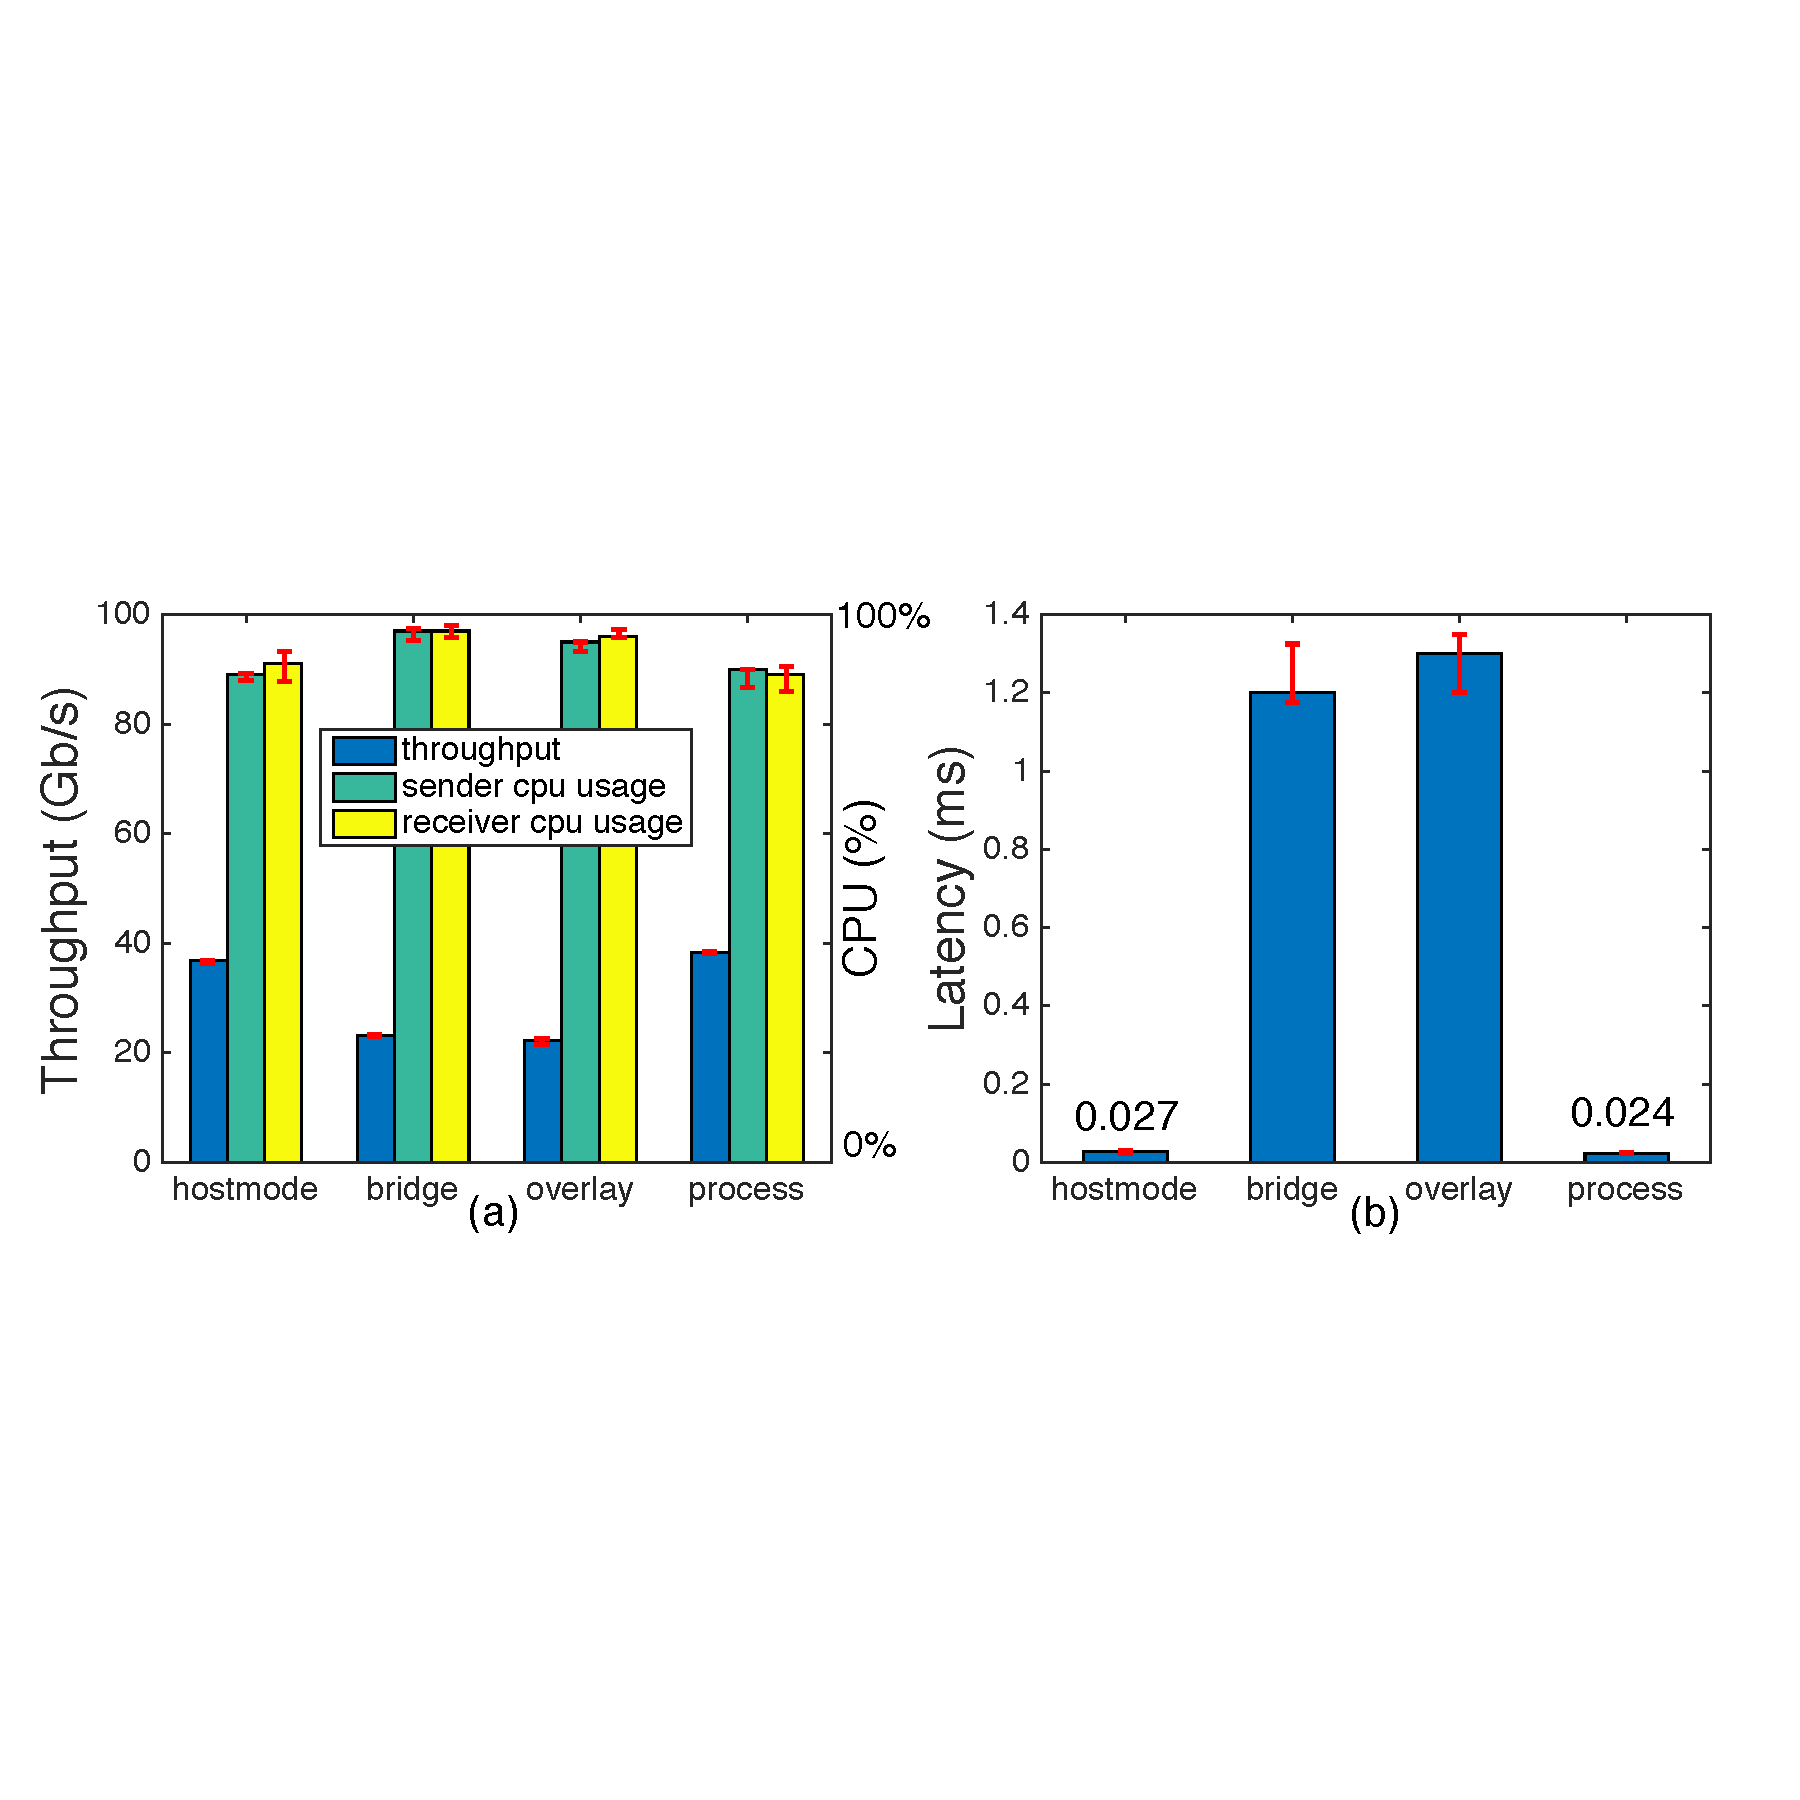
\includegraphics[width=0.5\textwidth]{figures/intro/intro_exist2.pdf} 
     \label{fig:three_modes}
     \caption{Performance of two modes of container networking, compared to
     shared memory IPC.} 
\end{figure} 

In addtion, we also consider a third mode, in which containers comunicate via
shared memory. This mode requires special configuration, and is the leat

Figure~\ref{fig:three_modes} shows the median network bandwidth and latency
between two containers in the two networking modes. The error bars show SIQR.

For contrast, the third bar shows the most performant way for two applications
on the same physical server: IPC communication via shared memory.  Note that
while containers do not have (easy) access to this mode of communication (even
though they are just processes), since they do not share the namespace.

We make two observations from this figure. First, that the throughput and
latency of both modes of inter-container communication is significantly worse
than shared-memory IPC. The reason is obvious: the container communication takes
a ``hairpin'' path through the full TCP/IP stack. Second,
the performance of overlay networking is worse than host mode. The reason, again,
is simple: in case of overlay networking, hairpinning happens twice, since the
packets must traverse through the software router as well. This figure thus
clearly illustrates the performance cost of isolation and portability.

As the popularity of container networking grows, this inefficiency must be
addressed. On one hand, the low throughput and high latency directly impacts
the overall performance of large scale distributed systems, such as big data
analytics~\cite{choudhury-paper}, key-value store~\cite{farm}, machine learning,
etc.  On the other hand, it forces the applications to reserve substantial CPU
resources to merely perform traffic processing, which significantly raise the
cost of running the applications.

It may seem that we have seen this movie before: virtualization suffers from
similar inefficiencies and we know how to address them using techniques like
SR-IOV~\cite{sriov} and NetVM~\cite{netvm}.

Unfortunately, these ideas cannot be directly applied to the container world.
SR-IOV typically scales to tens of VMs per server. In typical deployments, there
are hundreds of containers per server. The cost of supporting so many containers
in the NIC hardware will be prohibitive. 

NetVM~\cite{netvm} cannot be used directly with containers, since it destroys
portability -- it works only when two VMs are on the same server.
Developers prize containers especially for their portability: indeed, Docker's
main selling point is that a containerized application that runs on developer's
desktop will run in the cloud without any changes! 

In the above experiment, containers were on the same physical server. When
containers are on different physical servers, things become even trickier. For
example, such containers cannot easily use kernel bypass technologies like RDMA.
The reason is subtle: using RDMA (i.e. to bypass the kernel) direct access to
NICs is needed. This can only be done in the host mode -- since in the overlay
mode, the packets have to pass through the software router.  But operating in
the host mode means that containers on the same host share IP address, and must
carefully divvy up port space to avoid conflicts.  This limits their portability
-- e.g. there can be only one container bound to port 80 on each physical
server!

In this paper we outline a solution to address this issue.  Our ultimate vision
is to develop a container networking solution which provides high throughput,
low latency and negligible overhead and fully preserves container portability in
a manner that is completely transparent to application developers. 

To achieve these seemingly conflicting goals, we observe an opportunity to
leverage two key aspects of typical container deployments: (1) they are
typically managed by a central orchestrator (E.g., Mesos) and (2) are typically
deployed over managed network fabrics (e.g., a public cloud provider). Taking
advantage of these easily available additional bits of information, we sketch a
roadmap for an overlay-based solution  with flexible IP assignment and routing
in control-plane \vyas{why is this necessary} that obtains the relevant
deployment-specific information from the aforementioned container orchestrator
and fabric manager and use this in conjunction with the "right" I/O mechanism
(e.g., shared memory when containers are co-located, vs. RDMA when they are
not). 

While this sounds conceptually simple, there are several architectural
and system design challenges in realizing this vision in practice. In the rest
of the paper, we discuss these challenges and sketch a preliminary design. We
will also present results from an early prototype.
